\chapter{Basic Control}
\section{Introduction}
Basic control is a tupe of closed-loop control, with a single control loop. In this section, the transfer functions of the systems to be controlled are of first order or first order + deadtime. We will learn how to design PID controllers for this kind of systems.

The transfer functions that constitute the dynamics of the system to be controlled typically include two types:

Actuator transfer function. This usually corresponds to a flow control valve, steam valve, gas valve, etc.

Transfer functions of the plant (process). This is usually a first order transfer function of a tank, a boiler with heat exchanger, a reactor with heat exchanger, etc.

Controller. The objective of the basic control is to design a PID controller by cancellation of poles and zeros (analythical method) or by empirical methods (tables).

Process: a dynamic system with a particular purpose.

The goal of the control system is to correct deviations from the desired operation point.

\section{Controllers Design Methodology}
Controllers design is the central aspect of these sections and perhaps the most relevant aspect of the course. For this goal, two methodologies will be studied:
\begin{enumerate}
    \item Analytical design based on pole-zero cancellation
    \item Empirical design based on tables
\end{enumerate}
Depending on the system model we will select the corresponding option.

\subsection{Processes without delay}
In this case, analytical methods are applied. The main options are root locus analysis, the pole-zero cancellation method or the Ziegler Nichols (Z-N) tables for closed loop processes.

It is not possible to use other tables such as Open-loop Z-N or the AMIGO method.

Transfer function for the design of process controllers without delay:
\[\frac{K_p}{1 + t_p s}\]

Desging methods:
\begin{itemize}
    \item Closed-loop Z-N methods (applicable with or without delay)
    \item Analytical pole-zero cancellation design method (also known as direct synthesis).
\end{itemize}

\subsection{Processes with a delay}
These are controllers based on Ziegler Nichols (Z-N) tables and the AMIGO mehtod.

The design using Z-N tables or the AMIGO method, is fundamentally based on obtaining a first order function with a delay (First Order Plus Dead Time) of the process.

FOPDT model of the process:
\[\frac{K_p}{1 + t_p s} e^{-t_m s}\]
Where:
\begin{itemize}
    \item $K_p$: static gain
    \item $t_p$: time constant (or period)
    \item $t_m$: delay
\end{itemize}
A FOPDT model is representative of many types of processes.

Design methods:
\begin{itemize}
    \item Closed-loop Z-N method (applicable with or without process delay)
    \item Open-loop Z-N method (applicable with process delay)
    \item AMIGO method (applicable with process delay)
\end{itemize}

\section{Basic concepts of PID controller design}

PID (Proportional Integral Derivative) controllers are undoubtedly the most widely used in the industry. A PID controller is the result of combining three control actions: proportional action + derivative action + integral action.

\begin{figure}[H]
    \centering
    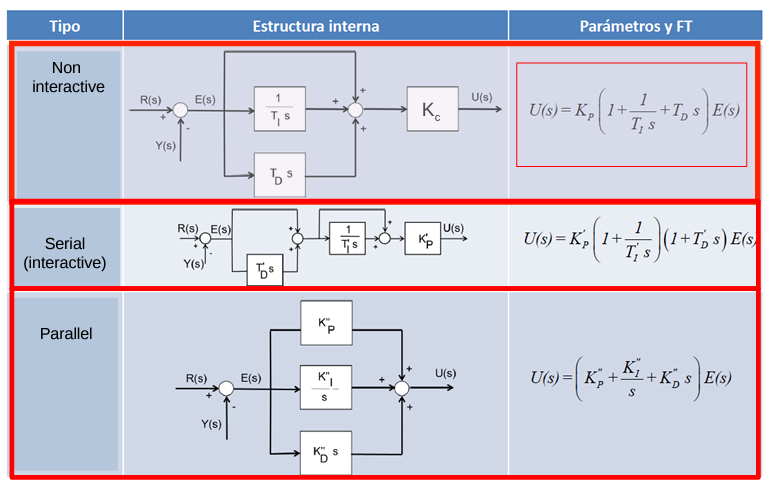
\includegraphics[width = 0.75 \textwidth]{Imagenes/3 - PID Types.png}
\end{figure}

\subsection{Proportional control: P}
Proportional control $K_p$ makes the response speed faster, which is desirable, but it increases the setling time.

A strong proportional control action increases the oscilation and inestability of the system. For safety reasons, overshooting should not exceed 30\%.

The proportional part does not consider time, therefore, the best way to solve the permanent error and consider the variation with respect to time, is to include and set the integral and derivative actions.